\documentclass[conference]{IEEEtran}
\usepackage[utf8]{inputenc}
\usepackage[T1]{fontenc}
\usepackage{cite}
\usepackage{graphicx}
\usepackage{booktabs}
\usepackage{url}
\usepackage{hyperref}
\hypersetup{hidelinks}
\renewcommand{\abstractname}{Resumen}
\renewcommand{\IEEEkeywordsname}{Palabras clave}

\title{Dise\~no e implementaci\'on de un monitor de recursos para Linux con Python, concurrencia y persistencia SQLite}

\author{
\IEEEauthorblockN{Julio Cesar Blacio Machuca \qquad Ariel Jose Llumiquinga \~Nacato}
\IEEEauthorblockA{Carrera de Ingenier\'ia de Software\\
Universidad de las Fuerzas Armadas ESPE\\
Sangolqu\'i, Ecuador}
}

\begin{document}

\maketitle

\begin{abstract}
La observaci\'on de recursos es una actividad esencial para comprender el estado de un sistema operativo, pero puede resultar abstracta cuando se estudia solo mediante comandos aislados. Este trabajo presenta el dise\~no y la implementaci\'on de una aplicaci\'on de terminal para Linux desarrollada en Python 3. La propuesta organiza seis m\'odulos de monitoreo mediante el patr\'on Modelo--Vista--Controlador: CPU, memoria y \textit{swap}, procesos, usuarios conectados, sistemas de archivos y red. Los datos se obtienen directamente del sistema de archivos virtual \texttt{/proc} y, cuando corresponde, de comandos nativos ejecutados de forma controlada. Como parte de los requisitos de sistemas operativos, la aplicaci\'on crea expl\'icitamente hilos con \texttt{threading.Thread} y un proceso hijo con \texttt{os.fork()}, cuya comunicaci\'on se realiza mediante una tuber\'ia. Las capturas completas se persisten en SQLite y se administran con operaciones CRUD. La verificaci\'on ejecutada en Ubuntu bajo WSL registr\'o 56 pruebas correctas, sin fallos. El resultado muestra una base did\'actica trazable que integra observaci\'on, concurrencia y persistencia sin sustituir las interfaces del sistema por dependencias de monitoreo de alto nivel.
\end{abstract}

\begin{IEEEkeywords}
Linux, monitoreo de recursos, Python, concurrencia, SQLite, sistema de archivos proc
\end{IEEEkeywords}

\section{Introducci\'on}
La administraci\'on de recursos permite relacionar la actividad de procesos, memoria, almacenamiento y comunicaciones con el comportamiento observable de un sistema operativo. En particular, los conceptos de procesos, planificaci\'on, memoria y entrada/salida requieren mecanismos concretos para pasar de la descripci\'on te\'orica a una observaci\'on verificable \cite{silberschatz2019}. Linux expone parte de ese estado mediante interfaces del n\'ucleo y comandos del espacio de usuario, lo que permite construir herramientas acotadas y transparentes para prop\'ositos formativos.

El proyecto \textit{Linux Resource Monitor} responde a esa necesidad con una aplicaci\'on interactiva de consola, orientada a observar y registrar el estado de un equipo Linux sin modificar procesos, red, memoria ni sistemas de archivos. Su alcance integra la lectura de recursos, la demostraci\'on expl\'icita de hilos y procesos, y la persistencia de capturas completas. No se plantea como sustituto de herramientas especializadas ni como medidor de rendimiento.

La contribuci\'on del trabajo es reunir en una sola aplicaci\'on de terminal el monitoreo de seis dominios, la lectura directa de \texttt{/proc}, comandos nativos, el uso expl\'icito de \texttt{threading.Thread} y \texttt{os.fork()}, y operaciones CRUD sobre SQLite. La estructura tambi\'en deja evidencia automatizada para que las afirmaciones funcionales puedan revisarse en Linux.

El objetivo t\'ecnico no se limita a enumerar valores: busca conservar la procedencia de cada dato desde la fuente del sistema hasta su presentaci\'on o almacenamiento. Para ello se definieron contratos estructurados entre capas, una pol\'itica de fallos parciales para la consulta en vivo y una regla m\'as estricta para persistir: una captura se guarda solamente cuando contiene los seis m\'odulos obligatorios. Esta distinci\'on permite observar un sistema cambiante sin confundir una vista incompleta con un registro hist\'orico completo.

\section{Fundamentos y trabajos relacionados}
El sistema de archivos virtual \texttt{/proc} publica informaci\'on generada por el n\'ucleo y por procesos en ejecuci\'on; por ello es una interfaz adecuada para consultar contadores y descriptores sin requerir una base de datos intermedia \cite{linuxproc}. En este trabajo se emplea para CPU, memoria, carga y tr\'afico de red, mientras que las sesiones, procesos y puntos de montaje se obtienen con utilidades nativas que presentan esas vistas del sistema.

Las dos clases de fuente tienen propiedades distintas. Los archivos de \texttt{/proc} representan el estado al momento de cada lectura, mientras que las utilidades producen una instant\'anea cuya composici\'on puede cambiar antes de que se presente. Por esta raz\'on, el dise\~no no exige que un conteo de procesos coincida despu\'es con otra ejecuci\'on de \texttt{ps}; exige registros bien formados y campos trazables. De igual manera, los contadores acumulados de red se conservan como bytes y paquetes, sin interpretarlos como tasas si no existe un intervalo de medici\'on.

Desde la perspectiva de sistemas operativos, separar la obtenci\'on, presentaci\'on y coordinaci\'on evita que el formato de la terminal se mezcle con el acceso a recursos. Esta decisi\'on facilita contrastar las mediciones, conservarlas como capturas y controlar los errores por m\'odulo. Adem\'as, permite estudiar la diferencia entre hilos que comparten el proceso y un hijo creado por \texttt{fork()}, sin ocultar esos mecanismos mediante bibliotecas de monitoreo de alto nivel \cite{silberschatz2019}.

\section{Metodolog\'ia}
\subsection{Desarrollo incremental}
El desarrollo se organiz\'o en cinco semanas. La primera defini\'o requerimientos, arquitectura MVC y esquema relacional; la segunda incorpor\'o CPU, memoria y lectura de \texttt{/proc}; la tercera agreg\'o disco, red, usuarios y procesos; la cuarta integr\'o hilos, \texttt{fork()} y CRUD; y la quinta se destin\'o a integraci\'on, pruebas, manuales y evidencias. Esta secuencia mantuvo cada avance asociado a una fuente de datos y a criterios de aceptaci\'on observables.

\subsection{Flujo de una captura}
Una solicitud de estado general atraviesa cuatro etapas. Primero, el controlador registra una funci\'on recolectora por m\'odulo. Segundo, el coordinador crea un objeto \texttt{Thread} para cada funci\'on, inicia los seis y espera su terminaci\'on. Tercero, consolida tres estructuras separadas: \texttt{datos}, \texttt{errores} y \texttt{evidencias}; esta \`ultima conserva nombre de m\'odulo, nombre de hilo e instantes UTC de inicio y fin. Finalmente, la vista puede presentar los datos disponibles y advertir los errores. Si el usuario decide registrar el estado, el controlador CRUD aplica una validaci\'on adicional antes de delegar la transacci\'on al repositorio.

La separaci\'on entre consulta y persistencia es deliberada. En una consulta en vivo, el fallo de una fuente no elimina la informaci\'on obtenida por las dem\'as. En cambio, \texttt{consolidar\_captura} verifica que existan CPU, memoria, discos, red, procesos y usuarios, y que el diccionario de errores est\'e vac\'io. Si falta un m\'odulo, se genera un error controlado y no se abre una operaci\'on de escritura para una captura incompleta.

\subsection{Fuentes y c\'alculos}
La CPU se describe con \texttt{/proc/cpuinfo}, \texttt{/proc/loadavg} y dos lecturas de \texttt{/proc/stat}. La utilizaci\'on no se infiere de la carga promedio: se calcula a partir de los deltas entre tiempo total e inactivo,
\begin{equation}
U_{CPU}=100\left(1-\frac{\Delta T_{idle}}{\Delta T_{total}}\right),
\end{equation}
donde ambos contadores proceden de la l\'inea agregada de CPU. Para memoria, se conserva la distinci\'on entre memoria libre y disponible: la memoria usada es \texttt{MemTotal - MemAvailable}, y el \textit{swap} usado es \texttt{SwapTotal - SwapFree}. La red usa \texttt{/proc/net/dev} para contadores e \texttt{ip} para direcciones; \texttt{ps}, \texttt{who} y \texttt{df -P -B1} complementan los datos de procesos, usuarios y sistemas montados.

\subsection{Contratos de datos}
Los modelos no devuelven bloques de terminal. CPU y memoria producen diccionarios; disco, red, procesos y usuarios producen listas de diccionarios, un elemento por montaje, interfaz, proceso o sesi\'on. Entre las claves estables se encuentran \texttt{porcentaje\_uso}, \texttt{mem\_disponible\_mb}, \texttt{punto\_montaje}, \texttt{usuario\_propietario}, \texttt{direccion\_ip} e \texttt{inicio\_sesion}. El controlador conserva estas estructuras y la vista es la responsable de agregar unidades, redondear a dos decimales y construir tablas ASCII.

Cada parser acepta texto y puede probarse sin consultar el equipo actual. La red combina los contadores de \texttt{/proc/net/dev} con una sola direcci\'on por interfaz: prioriza la primera IPv4 y usa IPv6 como alternativa; si no existe una direcci\'on, conserva \texttt{None}. El disco analiza bytes de \texttt{df -P -B1} antes de convertirlos para presentaci\'on o persistencia. En usuarios, \texttt{inicio\_sesion} mantiene el instante informado por \texttt{who}; la duraci\'on se calcula al mostrarlo y no reemplaza el dato almacenado.

\subsection{Concurrencia y seguridad}
Se crean seis hilos independientes, uno por m\'odulo, antes de esperar su finalizaci\'on. Los resultados, errores y evidencias se protegen con un bloqueo para consolidar una respuesta parcial cuando una lectura falla. Solo despu\'es de finalizar esos hilos se inicia el proceso hijo; este orden evita invocar \texttt{fork()} con otros hilos activos. El hijo lee una m\'etrica de carga, comunica un mensaje JSON por una tuber\'ia y el padre lo recolecta con \texttt{waitpid()}.

La demostraci\'on comprueba adem\'as que no existan otros hilos activos antes de crear el hijo. Padre e hijo cierran el extremo de la tuber\'ia que no utilizan; el hijo finaliza con \texttt{os.\_exit()} y el padre convierte el estado devuelto por \texttt{waitpid()} en un c\'odigo de salida. Un c\'odigo distinto de cero o una tuber\'ia vac\'ia se transforma en un error comprensible. La base de datos no participa en ese flujo y ninguna conexi\'on SQLite se comparte con hilos o con el proceso hijo.

\subsection{Fallos y estados cambiantes}
Los comandos se ejecutan con una lista de argumentos, salida y error capturados, modo texto, tiempo l\'imite de cinco segundos, \texttt{LC\_ALL=C} y sin \texttt{shell=True} \cite{pythonsubprocess}. Un retorno no nulo se convierte en \texttt{RuntimeError}; la ausencia de un comando, un tiempo agotado, un archivo de \texttt{/proc} inexistente o un contenido incompleto propagan una excepci\'on que el hilo registra con el nombre del m\'odulo. As\'i, el men\'u recibe mensajes controlados en lugar de una terminaci\'on abrupta.

Los parsers ignoran l\'ineas vac\'ias o no conformes cuando pueden continuar y rechazan campos obligatorios ausentes cuando el resultado perder\'ia significado. Este criterio es relevante para tablas que cambian durante la observaci\'on: un proceso puede terminar entre dos consultas y una interfaz puede carecer de IP. La aplicaci\'on admite listas vac\'ias y direcciones no disponibles, pero no inventa valores para completar la captura.

\subsection{Estrategia de verificaci\'on}
Las pruebas unitarias validan funciones de an\'alisis contra archivos de muestra para que los resultados no dependan solo de la m\'aquina actual. Las pruebas de persistencia usan bases SQLite temporales, incluyendo las operaciones CRUD y la eliminaci\'on en cascada. Las integraciones que requieren \texttt{fork()} se limitan expl\'icitamente a Linux. La ejecuci\'on documentada se realiz\'o en Ubuntu bajo WSL; por tanto, este art\'iculo no extiende esa evidencia a otros sistemas.

La verificaci\'on cubre tambi\'en contratos entre capas: que el controlador preserve errores parciales, que una captura incompleta sea rechazada, que las conexiones activen claves for\'aneas, que la actualizaci\'on afecte solo metadatos y que la eliminaci\'on retire las filas hijas. Para la interfaz se prueban opciones inv\'alidas, identificadores no positivos, cancelaci\'on de borrado, mensajes de \texttt{EXITO}, \texttt{ADVERTENCIA} y \texttt{ERROR}, y el l\'imite de listados extensos.

\section{Arquitectura y desarrollo de la soluci\'on}
\subsection{Separaci\'on MVC}
La Fig.~\ref{fig:arquitectura} resume la organizaci\'on. El modelo lee y transforma datos del sistema, y encapsula el repositorio SQLite. La vista solicita entradas por teclado y presenta men\'us, tablas y mensajes. El controlador coordina la recolecci\'on, las validaciones, la concurrencia y el flujo CRUD. Esta separaci\'on conserva contratos de datos estructurados entre capas y evita consultas SQL o lecturas de \texttt{/proc} en la vista.

La fachada \texttt{MonitorController} permite solicitar un m\'odulo o el estado general sin exponer c\'omo se obtiene. \texttt{CrudController} recibe el resultado concurrente, exige la captura completa y traduce errores de SQLite a una excepci\'on de aplicaci\'on. El repositorio es la \'unica pieza que conoce sentencias SQL; de esta forma, la navegaci\'on de terminal y las reglas de integridad pueden probarse mediante dobles sin ejecutar comandos Linux.

\begin{figure}[t]
\centering
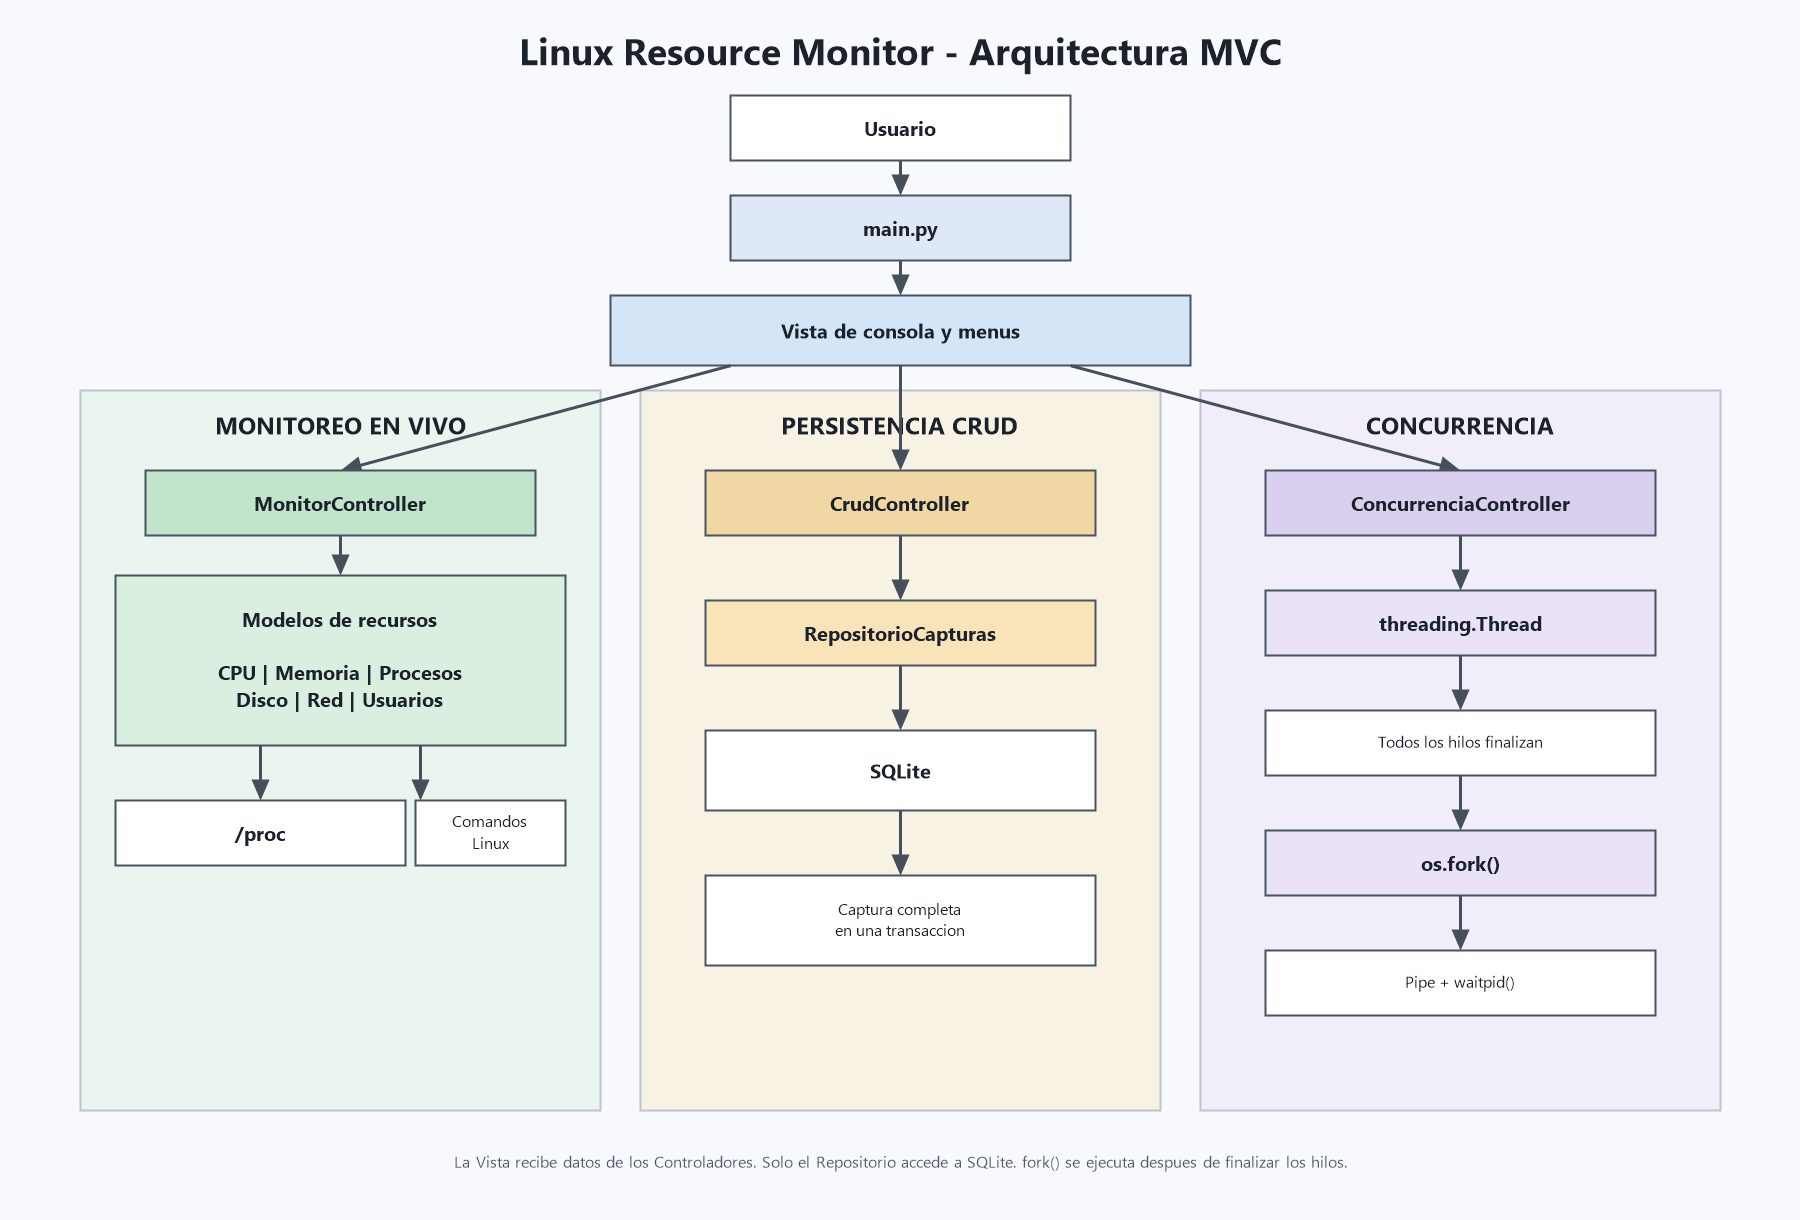
\includegraphics[width=\columnwidth]{figuras/arquitectura_actual.png}
\caption{Arquitectura MVC, recolecci\'on concurrente y persistencia del monitor.}
\label{fig:arquitectura}
\end{figure}

\subsection{M\'odulos de monitoreo}
La Tabla~\ref{tab:fuentes} relaciona cada m\'odulo con su fuente principal y el resultado que entrega al controlador. Las invocaciones de comandos se realizan con listas de argumentos, salida capturada, tiempo l\'imite y sin \texttt{shell=True}; el uso de \texttt{subprocess} conserva un l\'imite claro entre la aplicaci\'on y los comandos del sistema \cite{pythonsubprocess}. Las interfaces de Python usadas para procesos e hilos corresponden a las APIs documentadas de \texttt{os} y \texttt{threading} \cite{pythonos,pythonthreading}.

\begin{table}[t]
\caption{Trazabilidad entre m\'odulo, fuente y datos recolectados.}
\label{tab:fuentes}
\centering
\footnotesize
\begin{tabular}{@{}p{0.16\columnwidth}p{0.30\columnwidth}p{0.44\columnwidth}@{}}
\toprule
M\'odulo & Fuente principal & Datos obtenidos \\
\midrule
CPU & \texttt{/proc/cpuinfo}, \texttt{/proc/stat}, \texttt{/proc/loadavg} & Procesadores l\'ogicos, modelo, frecuencia, carga y uso \\
Memoria & \texttt{/proc/meminfo} & Total, libre, disponible, usada y \textit{swap} \\
Procesos & \texttt{ps} & PID, nombre, estado y propietario \\
Usuarios & \texttt{who} & Usuario, terminal e inicio de sesi\'on \\
Disco & \texttt{df -P -B1} & Punto de montaje, bytes y porcentaje de uso \\
Red & \texttt{/proc/net/dev}, \texttt{ip} & Interfaz, direcci\'on y contadores de tr\'afico \\
\bottomrule
\end{tabular}
\end{table}

El m\'odulo de CPU separa carga y utilizaci\'on: las tres cargas provienen de \texttt{/proc/loadavg}, mientras que el porcentaje usa los deltas de \texttt{/proc/stat}. El conteo se denomina procesadores l\'ogicos porque surge de las entradas \texttt{processor} de \texttt{/proc/cpuinfo}; no se presenta como n\'ucleos f\'isicos. En memoria se validan cinco campos obligatorios antes de convertir de KiB a MiB. Para procesos, usuarios y disco se analiza una ejecuci\'on de \texttt{ps}, \texttt{who} o \texttt{df}, respectivamente, lo que conserva una instant\'anea coherente con la fuente invocada.

\subsection{Concurrencia y persistencia}
La recolecci\'on inicia los seis objetos \texttt{Thread}, los une antes de consolidar el resultado y conserva errores por m\'odulo. El proceso hijo se crea mediante \texttt{os.fork()}, env\'ia sus datos por \texttt{pipe} y se recolecta sin dejar procesos hu\'erfanos. Esta secuencia hace visible la diferencia entre coordinaci\'on de hilos y comunicaci\'on entre procesos.

Las capturas se almacenan en una tabla principal con m\'etricas relacionadas de CPU, memoria, disco, procesos, red y usuarios. Cada conexi\'on activa las claves for\'aneas y cada captura completa se escribe en una transacci\'on, de modo que un fallo requerido revierte la operaci\'on. Las relaciones usan eliminaci\'on en cascada para retirar las m\'etricas asociadas cuando se elimina una captura \cite{sqlitefk,sqlitetransactions}. El CRUD permite crear, listar y consultar capturas, actualizar sus metadatos y eliminarlas mediante el repositorio.

El dise\~no relacional distingue cardinalidades. CPU y memoria tienen una relaci\'on uno a uno con \texttt{capturas}: su clave primaria es tambi\'en clave for\'anea. Disco, procesos, red y usuarios tienen relaciones uno a muchos y claves propias, porque una captura puede incluir varios elementos de cada tipo. La tabla padre conserva fecha, etiqueta, comentario y usuario de registro; la operaci\'on de actualizaci\'on modifica solo etiqueta y comentario, nunca las m\'etricas observadas.

La escritura abre una conexi\'on independiente y entra en el contexto transaccional antes de insertar la fila padre y las seis familias de m\'etricas. Si una clave requerida no existe, un tipo de contrato es incorrecto o SQLite rechaza una fila, el contexto revierte el conjunto y el bloque \texttt{finally} cierra la conexi\'on. En la lectura, el repositorio reconstruye el mismo contrato empleado por la vista: un diccionario para CPU y memoria, y listas para las relaciones uno a muchos.

\subsection{Criterios de interfaz terminal}
El men\'u principal y el historial se operan con opciones numeradas. Una entrada inv\'alida conserva el bucle activo; los identificadores deben ser enteros positivos y la eliminaci\'on exige escribir \texttt{SI}. Los listados de procesos y sistemas de archivos se limitan inicialmente a 20 filas e indican cu\'antos registros se muestran respecto del total. Estas decisiones evitan que una instant\'anea extensa desplace indefinidamente el contexto de la terminal.

La salida no depende del color. Los porcentajes se acompa\~nan con \texttt{NORMAL}, \texttt{ADVERTENCIA} o \texttt{CRITICO}; los valores incluyen unidades y dos decimales, y el estado general muestra fecha de actualizaci\'on. Las ausencias se expresan como \emph{No disponible} o mediante mensajes espec\'ificos para listas vac\'ias. Por ello, la interfaz sigue siendo comprensible en una terminal de texto simple y mediante teclado.

\section{Resultados y validaci\'on}
La Tabla~\ref{tab:resultados} resume una ejecuci\'on verificada el 12 de julio de 2026 en Ubuntu bajo WSL. La suite se ejecut\'o con \texttt{python3 -m unittest discover -s tests}; los dem\'as registros aplicaron el controlador de monitoreo, un repositorio SQLite temporal y la demostraci\'on de concurrencia. Los valores son una instant\'anea de verificaci\'on funcional, no un punto de referencia de rendimiento ni una comparaci\'on de plataformas.

\begin{table}[t]
\caption{Resultados verificados de la ejecuci\'on documentada.}
\label{tab:resultados}
\centering
\footnotesize
\begin{tabular}{@{}p{0.25\columnwidth}p{0.43\columnwidth}p{0.20\columnwidth}@{}}
\toprule
Validaci\'on & Resultado & Estado \\
\midrule
Suite completa & 56 pruebas & 0 fallos \\
Estado general & 6 m\'odulos & 0 errores \\
CRUD SQLite & Crear/listar/actualizar/eliminar & Correcto \\
Concurrencia & 6 hilos + 1 hijo & Exit status 0 \\
\bottomrule
\end{tabular}
\end{table}

La evidencia de estado general registr\'o los m\'odulos CPU, memoria, discos, procesos, red y usuarios, con un diccionario de errores vac\'io. En la prueba de persistencia se cre\'o una captura, se list\'o, se actualizaron sus metadatos y se elimin\'o; el listado final qued\'o sin registros. En la demostraci\'on de concurrencia se generaron seis evidencias con nombres \texttt{monitor-} y marcas de inicio y fin, seguidas de un hijo con PID distinto al padre y c\'odigo de salida cero.

La suite combina pruebas deterministas y verificaciones de integraci\'on. Los parsers de CPU, memoria, disco, red, procesos y usuarios consumen archivos de muestra; el repositorio se crea en un directorio temporal y comprueba tanto el detalle reconstruido como la cascada; los controladores se ejercitan con recolectores y repositorios sustituibles; y los casos de Linux validan el flujo integrado y el \texttt{fork()} real. Esta composici\'on reduce la dependencia de valores ef\'imeros sin eliminar la comprobaci\'on final sobre el sistema objetivo.

Los criterios de aceptaci\'on se interpretaron seg\'un la naturaleza de cada dato. Se exige igualdad de claves y f\'ormulas para CPU y memoria, registros parseables para comandos, una direcci\'on primaria o ausencia expl\'icita en red, continuidad ante fallos parciales para la vista en vivo y atomicidad para el historial. No se exige igualdad exacta entre conteos tomados en instantes diferentes ni se generalizan los tiempos observados en una ejecuci\'on.

\begin{figure}[t]
\centering
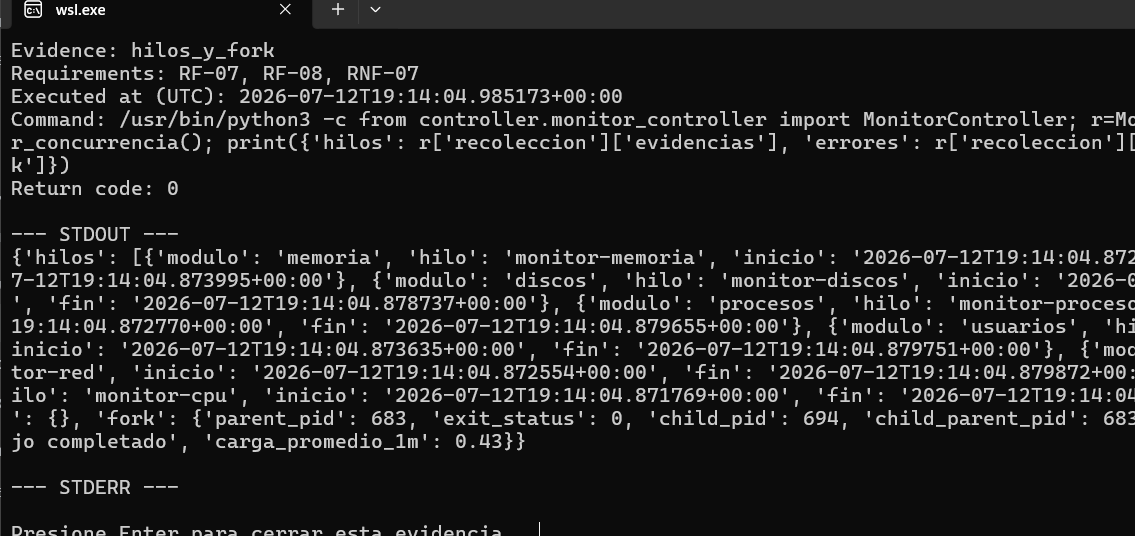
\includegraphics[width=\columnwidth]{figuras/evidencia_hilos_fork.png}
\caption{Evidencia de la ejecuci\'on de seis hilos y un proceso hijo en WSL.}
\label{fig:concurrencia}
\end{figure}

\section{Conclusiones}
El monitor integra los requisitos funcionales de observaci\'on de CPU, memoria, procesos, usuarios, disco y red en una aplicaci\'on de terminal para Linux. La separaci\'on MVC mantiene diferenciadas la lectura de recursos, la coordinaci\'on y la presentaci\'on; a su vez, el repositorio concentra la persistencia y las operaciones CRUD sobre SQLite.

La demostraci\'on de seis hilos y un hijo ilustra una decisi\'on de orden relevante: los hilos terminan antes de iniciar \texttt{fork()}, y el padre recupera al hijo mediante una tuber\'ia y \texttt{waitpid()}. La transacci\'on para cada captura completa y las claves for\'aneas con cascada sostienen la consistencia de los datos almacenados. La verificaci\'on documentada respalda el comportamiento descrito, sin atribuirle propiedades de rendimiento.

Como limitaciones, las lecturas dependen de las interfaces Linux disponibles y representan estados cambiantes del sistema. Trabajos futuros pueden estudiar la portabilidad de la capa de obtenci\'on o muestras de mayor duraci\'on, conservando la separaci\'on arquitect\'onica y sin afirmar que dichas extensiones formen parte de la versi\'on actual.

\bibliographystyle{IEEEtran}
\bibliography{referencias}

\end{document}
